% --- ARCHIVO: Cap6_Impacto_Comunicativo/impacto_comunicativo.tex ---

\chapter{Impacto Socio-Comunicativo y Tratamiento Informativo}
\label{cap:impacto_comunicativo}

\section{Análisis de prensa: identificación de sesgos técnicos y
narrativa mediática sobre los responsables del apagón}
\label{sec:analisis_prensa}

\lettrine[lines=3, lhang=0.1]{L}{a} gestión comunicativa del apagón del 28 de abril de 2025 constituyó
un caso relevante de lo que la literatura especializada denomina
\textit{crisis communication
failure}\textsuperscript{\ref{anexo:crisis_comm_failure}}: la
incapacidad de las instituciones para ocupar el espacio informativo
con mensajes técnicos verificables en el intervalo temporal crítico
que sigue a un incidente de infraestructura \cite{mitceepr2025}. El
cero de tensión peninsular se produjo a las 12:33~CEST; la primera
comparecencia pública oficial del presidente del Gobierno no tuvo
lugar hasta las 18:00~CEST, más de cinco horas después. En ese
intervalo, el ecosistema hiperconectado ---súbitamente privado de
suministro eléctrico y, con él, de acceso digital--- procesó la
emergencia en ausencia de cualquier marco interpretativo
institucional.

Este vacío fue ocupado de forma inmediata por lo que la Organización
Mundial de la Salud ha denominado
\textit{infodemia}\textsuperscript{\ref{anexo:infodemia}}: la
propagación de información no verificada que se acelera en contextos
de incertidumbre extrema y privación sensorial \cite{blackswan2025}.
Hipótesis de sabotaje, ciberataques de origen ruso, fenómenos
atmosféricos anómalos y experimentos gubernamentales con el sistema
eléctrico circularon a escala global antes de que los operadores del
sistema emitieran un diagnóstico preliminar. La naturaleza del
incidente ---un colapso por sobretensión cuya mecánica física, como
se ha analizado en la sección~\ref{sec:discrepancias}
(p.~\pageref{sec:discrepancias}), requiere conocimientos de
estabilidad de tensión, comportamiento de Recursos Basados en
Inversores (IBR) y dinámica de Cambiadores de Tomas en Carga (OLTC)
para ser comprendida--- lo hacía especialmente vulnerable a esta
dinámica: la complejidad técnica del fenómeno real era inversamente
proporcional a la accesibilidad de las explicaciones alternativas que
lo sustituyeron en el espacio público.

La consecuencia documentada de este proceso fue la incorporación del
incidente al debate político sobre la transición energética antes de
que se dispusiera de un diagnóstico técnico verificado. En un contexto
en que el debate sobre el modelo de operación del sistema eléctrico
funcionaba ya como eje de discusión pública, el apagón fue encuadrado
de forma inmediata en categorías interpretativas preexistentes. El
resultado, documentado a continuación mediante el análisis de la
cobertura mediática y la actividad en redes sociales, fue que la
opinión pública española recibió durante semanas explicaciones
causales ---``las renovables causaron el apagón'', ``faltaron
nucleares'', ``Europa abandonó a España''--- que los cuatro informes
técnicos analizados en el capítulo~\ref{cap:analisis_informes}
(p.~\pageref{cap:analisis_informes}) no respaldan de forma unánime
\cite{gobierno2025,ree2025,entsoe2025}. La distancia entre el consenso
técnico y la narrativa mediática dominante es, en sí misma, una de
las consecuencias del 28 de abril de 2025 con implicaciones directas
sobre la capacidad de la sociedad para evaluar las reformas
regulatorias que el incidente pone de manifiesto.

% - - - - - - - - - - - - - - - - - - - - - - - - - - - - - - - - -
\subsection*{La prensa crítica con la gestión institucional}
% - - - - - - - - - - - - - - - - - - - - - - - - - - - - - - - - -

Cabeceras como El~Mundo, ABC y La~Razón articularon una narrativa que
vinculaba el colapso del sistema con la gestión energética del
Gobierno, interpretando el apagón como consecuencia previsible de una
transición energética que habría priorizado la penetración de fuentes
intermitentes sin garantizar mecanismos de respaldo suficientes. Este
encuadre presenta inconsistencias verificables con las conclusiones de
los informes técnicos analizados en el
capítulo~\ref{cap:analisis_informes}
(p.~\pageref{cap:analisis_informes}).

El~Mundo publicó el titular ``\textit{La red eléctrica sufría ya `anomalías
críticas´$ $  a nivel nacional al menos media hora antes del gran apagón}'',
encuadrando el incidente como consecuencia de señales de alerta
desatendidas operativamente. El diario conectó el argumento técnico
de la debilidad de las interconexiones con la narrativa de
responsabilidad institucional por el modelo energético
\cite{mitceepr2025}. Posteriormente publicó ``\textit{Flamanville~3 y las 56
nucleares francesas que salvaron al antinuclear Sánchez durante el
gran apagón}'', atribuyendo implícitamente la reposición del suministro
a la tecnología nuclear, y ``\textit{Sánchez también se apaga}'', en un
encuadre que personalizaba la responsabilidad en el presidente.

ABC centró parte de su análisis en la inercia rodante. Columnas de
opinión afirmaban que la red se encontraba ``\textit{a un papel de fumar}'' de
colapsar por la ``\textit{alarmante falta de inercia rotacional provocada por
las centrales nucleares apagadas}''. El diario tituló el 30 de abril
``\textit{La falta de energía nuclear y el `boom´ renovable fulminaron
la red}'', y su editorial del 5 de mayo afirmó que ``\textit{el Gobierno
conocía el riesgo de apagones desde marzo}'' y que la vicepresidenta
``\textit{no se tomó en serio los avisos}''. La afirmación sobre la inercia
entra en contradicción con el consenso técnico expuesto en la
sección~\ref{sec:discrepancias}
(p.~\pageref{sec:discrepancias}): los registros oficiales certifican
que, en el momento del colapso, la red contaba con una inercia del
sistema de $H = 2,3$~s, por encima del umbral recomendado por
ENTSO-E, confirmando que el evento no fue un colapso por déficit de
masa síncrona sino un fenómeno de inestabilidad capacitiva
\cite{icai2025,entsoe2025}.

La figura~\ref{fig:collage_conservador} recoge una muestra
representativa de la cobertura de este bloque mediático. El análisis
del encuadre periodístico
(\textit{framing})\textsuperscript{\ref{anexo:framing}} permite
identificar un patrón de atribución de responsabilidades a la
política energética del Ejecutivo, apoyado en argumentos causales
que los informes periciales respaldaron solo de forma parcial.

\begin{figure}[H]
    \centering
    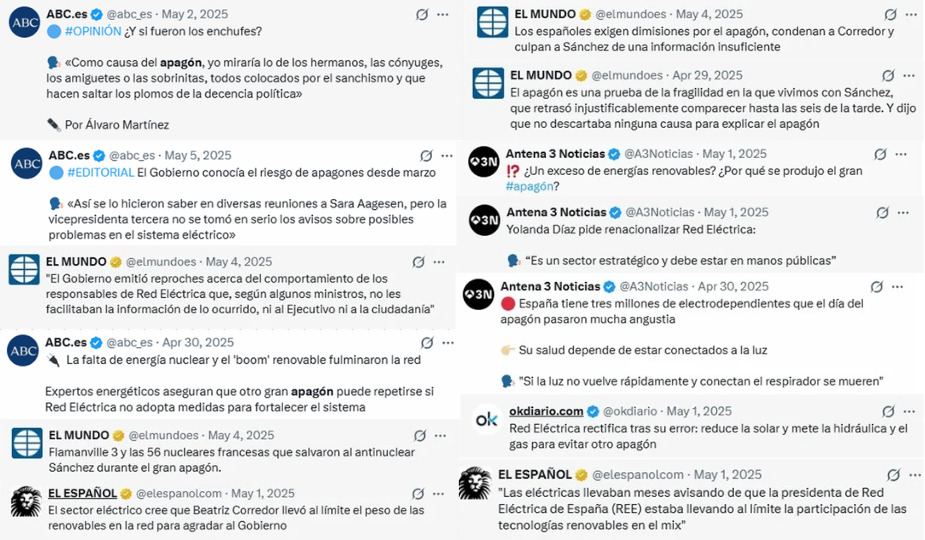
\includegraphics[width=\textwidth]{figuras/collage_conservador.png}
    \vspace{0.2cm}
    \caption[Muestra de portadas y publicaciones de medios críticos
    con la gestión institucional.]{%
    Muestra representativa de portadas y publicaciones en medios con
    postura crítica frente a la gestión institucional del incidente.
    Fuente: Elaboración propia a partir de publicaciones en X}
    \label{fig:collage_conservador}
\end{figure}


La Razón publicó la portada ``\textit{Caos total}'' y se hizo eco de
peritajes independientes con el titular: ``\textit{Un informe preliminar
concluye que la programación de insuficiente generación síncrona con
control dinámico de tensión fue la causa del apagón}''. Esta
afirmación encuentra respaldo parcial en los análisis técnicos: el
déficit de capacidad de absorción de potencia reactiva en la zona sur
fue, efectivamente, uno de los factores identificados en el peritaje
del IIT-ICAI \cite{icai2025}. Sin embargo, el mismo informe señala
que ese déficit se produjo en un contexto en que las maniobras del
Operador del Sistema habían inyectado previamente una cantidad
significativa de reactiva capacitiva, factor que la cobertura de este
bloque no incorporó de forma sistemática.

En términos agregados, la cobertura de los medios críticos con la
gestión institucional puede describirse como una reducción de un
fenómeno multicausal ---que incluye el \textit{mallado}, el
\textit{Tap-Lag} y el \textit{Efecto Ferranti}--- a una relación
causal de tipo ``\textit{mayor penetración renovable --- menor estabilidad
--- apagón}''. El panel de expertos de ENTSO-E señaló explícitamente
que el evento no se debió a un exceso de renovables \textit{per se} sino a la
obsolescencia de los códigos de red que impedían a los IBR participar
activamente en el control de tensión \cite{entsoe2025}.

% - - - - - - - - - - - - - - - - - - - - - - - - - - - - - - - - -
\subsection*{La prensa con postura favorable a la narrativa institucional}
% - - - - - - - - - - - - - - - - - - - - - - - - - - - - - - - - -

Los medios con postura favorable a la narrativa institucional
desplazaron el foco desde las tecnologías renovables hacia la gestión
operativa de REE, las carencias estructurales de la red de transporte
y las políticas heredadas de administraciones anteriores. La premisa
articuladora fue que el colapso no constituyó un fracaso de la
descarbonización sino el resultado de una infraestructura no
modernizada al ritmo necesario. Esta tesis encuentra respaldo parcial
en los informes periciales, aunque en ocasiones fue articulada
omitiendo factores causales relevantes o incorporando atribuciones de
responsabilidad sin respaldo técnico directo \cite{gobierno2025}.

El País destacó que la capacidad de intercambio con Francia se
sitúa en un 3~\%, muy inferior al objetivo europeo del 15~\%,
señalando una inversión  en la interconexión transfronteriza históricamente insuficiente. Este
argumento es técnicamente consistente con los informes: de haber
existido mayor capacidad de interconexión, la probabilidad y
virulencia de las oscilaciones inter-área habrían sido menores
\cite{entsoe2025}. Por su parte, elDiario.es señaló que REE operó
con márgenes de seguridad reducidos a pesar de la previsión de alta
radiación solar y baja generación síncrona. Esta afirmación es
coherente con el diagnóstico sobre el déficit de potencia reactiva en
el sur documentado en el peritaje de IIT-ICAI, aunque la cobertura
no articuló el mecanismo técnico subyacente de la saturación de las
curvas Q-V \cite{icai2025}.

La figura~\ref{fig:collage_progresista_redes} recoge una muestra
representativa de este bloque mediático. Al igual que en el bloque
crítico, la cobertura respondió al \textit{framing} como mecanismo
de reducción de la ambigüedad cognitiva ante un fenómeno de elevada
complejidad técnica.

\vspace{0.6cm}
\begin{figure}[H]
    \centering
    
\includegraphics[width=\textwidth]{figuras/collage_progresista.png}
    \vspace{0.2cm}
    \caption[Muestra de publicaciones en medios con postura favorable
    a la narrativa institucional.]{%
    Muestra representativa de publicaciones en redes sociales
    asociadas a medios con postura favorable a la narrativa
    institucional. Fuente: Elaboración propia a partir de
    publicaciones en X}
    \label{fig:collage_progresista_redes}
\end{figure}
\vspace{0.6cm}

En este bloque se identifican también desviaciones respecto al
consenso técnico. La Vanguardia publicó que los mecanismos de
protección continentales actuaron de forma ``egoísta'' al desconectar
a la Península para salvaguardar el suministro en Francia. Esta
caracterización entra en contradicción con el dictamen de ENTSO-E: la
apertura transpirenaica a las 12:33:21~CEST fue la actuación
automática de las protecciones de pérdida de sincronismo (OST) ante
una divergencia angular severa \cite{entsoe2025}. Atribuir un carácter
deliberado a la actuación de un mecanismo de protección automático
supone una confusión entre el funcionamiento de las protecciones del
sistema y una decisión operativa consciente.

Por su parte, medios como infoLibre publicaron que los operadores
privados fallaron deliberadamente al no absorber la tensión excedente.
Esta lectura incorpora la acusación de ``indisciplina técnica'' del
Gobierno pero omite el factor que el peritaje de IIT-ICAI sitúa
cronológicamente antes: la maniobra de mallado del Operador del
Sistema que inyectó potencia reactiva capacitiva en la red antes de
que se produjera ningún disparo \cite{icai2025}. La selección parcial
de los factores causales es aquí simétrica a la identificada en el
bloque crítico con la gestión institucional: cada bloque mediático
incorporó los hechos consistentes con su encuadre previo y omitió
aquellos que lo contradecían.

% - - - - - - - - - - - - - - - - - - - - - - - - - - - - - - - - -
\subsection*{La cobertura internacional: encuadre estructural europeo}
% - - - - - - - - - - - - - - - - - - - - - - - - - - - - - - - - -

La prensa internacional abordó el apagón desde una perspectiva
estructural. Al no participar del debate político español, las
cabeceras de referencia internacionales encuadraron el cero de
tensión como un fallo sistémico de la arquitectura de redes europeas
y como advertencia para sistemas con alta penetración de electrónica
de potencia. Esta perspectiva no estuvo, sin embargo, exenta de
inexactitudes técnicas.

\vspace{0.6cm}
\begin{figure}[H]
    \centering
    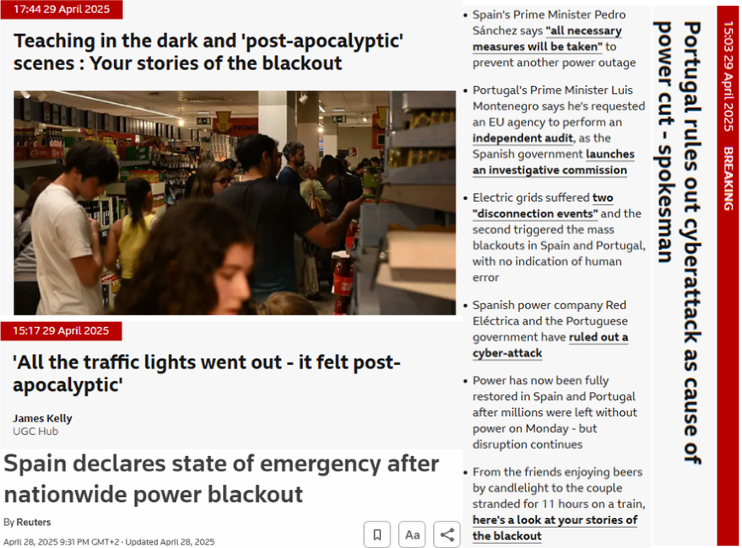
\includegraphics[width=\textwidth]{figuras/collage_internacional.png}
    \vspace{0.2cm}
    \caption[Muestra de la cobertura en medios internacionales.]{%
    Muestra representativa de la cobertura del incidente en medios
    de comunicación internacionales.
    Fuente: Elaboración propia}
    \label{fig:collage_internacional}
\end{figure}
\vspace{0.6cm}

Reuters proporcionó un análisis con mayor rigor técnico, destacando
el papel de las interconexiones y el déficit de soporte de tensión de
las centrales convencionales en los instantes previos al colapso
\cite{ree2025}. Le~Monde adoptó un enfoque descriptivo del impacto
transfronterizo y la BBC centró su cobertura en la seguridad de las
infraestructuras críticas, documentando la parada segura de los
reactores nucleares y refutando las hipótesis de ciberataque.

Financial~Times tituló ``\textit{Spain and Portugal blackout blamed on
solar power dependency}'', citando expertos que atribuían la
inestabilidad a la insuficiencia de ``\textit{firm power}''. Esta
argumentación no se corresponde con el consenso técnico: el sistema
contaba con reservas operativas suficientes y cuatro reactores
nucleares acoplados en el momento del incidente \cite{entsoe2025}. El
evento no fue un colapso de potencia activa por falta de generación
firme sino un fenómeno de inestabilidad de tensión capacitiva.

La desviación más documentada provino de The~Telegraph, cuya portada
sugirió que el Gobierno español realizaba un ``\textit{experimento}'' con el
sistema eléctrico. Esta afirmación fue desmentida por las plataformas
de verificación Euronews~Verify y Reuters~Fact~Check y no encontró
respaldo en ninguno de los cuatro informes técnicos analizados.

% - - - - - - - - - - - - - - - - - - - - - - - - - - - - - - - - -
\subsection*{Síntesis: selección asimétrica de evidencias y
polarización del debate energético}
% - - - - - - - - - - - - - - - - - - - - - - - - - - - - - - - - -

La conclusión que arroja este análisis comunicativo es que el
incidente no fue cubierto mayoritariamente como un fenómeno técnico
novedoso sino encuadrado de forma inmediata en los marcos
interpretativos preexistentes de cada bloque editorial. Coherente
con la teoría del \textit{framing} mediático, los medios redujeron
la ambigüedad cognitiva ante un fenómeno de alta complejidad técnica
a expensas de la precisión analítica \cite{mitceepr2025}.

La consecuencia directa fue la \textit{selección asimétrica de
evidencias}: los medios críticos con la gestión institucional
enfatizaron el déficit de generación síncrona y la política energética
como causas, con omisión frecuente del impacto del mallado; los medios
con postura favorable a la narrativa oficial enfatizaron el error
operativo y el déficit de interconexiones, con omisión frecuente del
comportamiento real del parque de generación. El resultado fue que
ninguno de los dos bloques ofreció una representación de la
multicausalidad técnica tal como ha sido descrita en los informes
periciales \cite{icai2025,gobierno2025}.

Esta dinámica tiene implicaciones que exceden el análisis mediático.
Las reformas técnicas y regulatorias identificadas como necesarias por
los informes ---actualización del P.O.~7.4, despliegue de
compensadores síncronos, transición al modo \textit{grid-forming}---
requieren un nivel de consenso político sostenido. La polarización del
debate público en torno a narrativas causales mutuamente excluyentes
dificulta la formación de ese consenso.

% ---------------------------------------------------------------------
\section{Reacción en redes sociales: gestión de la incertidumbre,
desinformación y percepción de la emergencia}
\label{sec:redes_sociales}
% ---------------------------------------------------------------------

El análisis de la actividad en la plataforma X durante el apagón
revela una evolución secuencial en tres fases: una fase de
incertidumbre aguda (0--6~horas), dominada por la desinformación y los
mecanismos de afrontamiento colectivo; una fase de politización
(6--72~horas), caracterizada por la consolidación de narrativas de
atribución de responsabilidad; y una fase de corrección tardía en la
que las explicaciones técnicas llegaron con alcance significativamente
inferior al de los mensajes iniciales \cite{mitceepr2025}.

% - - - - - - - - - - - - - - - - - - - - - - - - - - - - - - - - -
\subsection*{La fase de incertidumbre aguda (0--6 horas):
desinformación e hipótesis alternativas}
% - - - - - - - - - - - - - - - - - - - - - - - - - - - - - - - - -

La ausencia de comunicación gubernamental durante las primeras cinco
horas generó un proceso de \textit{vacuum
filling}\textsuperscript{\ref{anexo:vacuum_filling}}: el vacío
informativo fue ocupado por fuentes no verificadas \cite{blackswan2025}.
La elevada opacidad técnica del colapso por sobretensión favoreció la
propagación de hipótesis de sabotajes, ciberataques (la denominada
«Operación Matrioska») y fenómenos atmosféricos. Todas ellas resultaron
fácilmente asimilables por el público general debido a su narrativa
externaliza\-dora.

Superpuesta a este ecosistema desinformativo, emergió una respuesta
ciudadana coherente con la \textit{emergent norm
theory}\textsuperscript{\ref{anexo:emergent_norm}}: el desarrollo
de mecanismos colectivos de afrontamiento ante la perturbación. El
humor costumbrista, la ironía y la normalización pragmática de la
situación funcionaron como reguladores emocionales colectivos ante
una disrupción de amplitud sin precedentes en España.

La figura~\ref{fig:collage_ciudadanos} recoge una muestra de las
publicaciones ciudadanas durante las primeras horas. Se identifican
tres patrones de respuesta: la normalización pragmática y el humor
costumbrista como mecanismo de afrontamiento, la crítica institucional
a través de formatos virales, y la búsqueda activa de explicaciones
causales en ausencia de información oficial. Los tres patrones son
coherentes con la \textit{emergent norm theory} aplicada a entornos
digitales en situaciones de disrupción de infraestructuras críticas.

\begin{figure}[H]
    \centering
    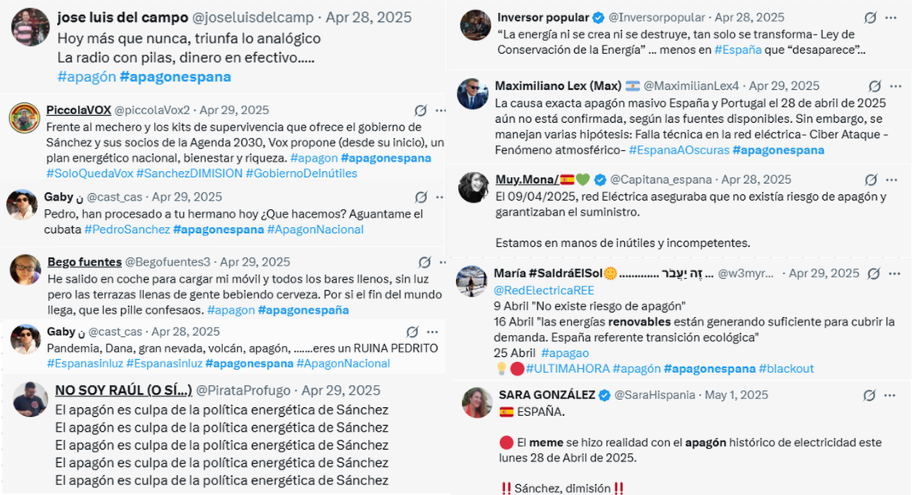
\includegraphics[width=\textwidth]{figuras/collage_ciudadanos.png}
    \vspace{0.2cm}
    \caption[Reacciones ciudadanas en X durante las primeras horas
    del apagón (28--29~de~abril~de~2025).]{%
    Muestra representativa de publicaciones de usuarios sin
    afiliación mediática institucional identificable en la plataforma
    X durante las primeras horas del incidente.
    Fuente: capturas de X, elaboración propia}
    \label{fig:collage_ciudadanos}
\end{figure}


% - - - - - - - - - - - - - - - - - - - - - - - - - - - - - - - - -
\subsection*{La politización del discurso (6--72 horas): encuadres
de atribución}
% - - - - - - - - - - - - - - - - - - - - - - - - - - - - - - - - -

A partir de la comparecencia oficial, el discurso digital migró hacia
la atribución de responsabilidades, un proceso catalogado como
\textit{outrage
communication}\textsuperscript{\ref{anexo:outrage_comm}} en la
literatura de comunicación de crisis, en el que los mensajes de
indignación generan mayor capacidad de difusión algorítmica que las
explicaciones técnicas \cite{mitceepr2025}.

En el espacio digital con postura crítica frente al Gobierno, el
apagón fue encuadrado como evidencia de una gestión deficiente.
Figuras políticas publicaron exigencias de dimisiones y rendición de
cuentas y reivindicaron protocolos de seguridad adoptados por otras
administraciones. En el espacio digital con postura favorable a la
narrativa institucional, la línea argumentativa se orientó hacia la
valoración positiva de la respuesta del sistema de emergencias y la
defensa del modelo energético vigente, frente a las críticas
formuladas por el bloque contrario.

La figura~\ref{fig:collage_politicos} recoge una muestra de las
publicaciones de figuras políticas. Al igual que en la cobertura de
prensa, se observa que ninguno de los mensajes analizados abordó aspectos técnicos del colapso por sobretensión, del fenómeno del
\textit{Tap-Lag} o del papel del mallado. La comunicación política de ambas
posiciones se orientó a la atribución de responsabilidades sin
incorporar los elementos técnicos centrales del diagnóstico pericial.

\begin{figure}[H]
    \centering
    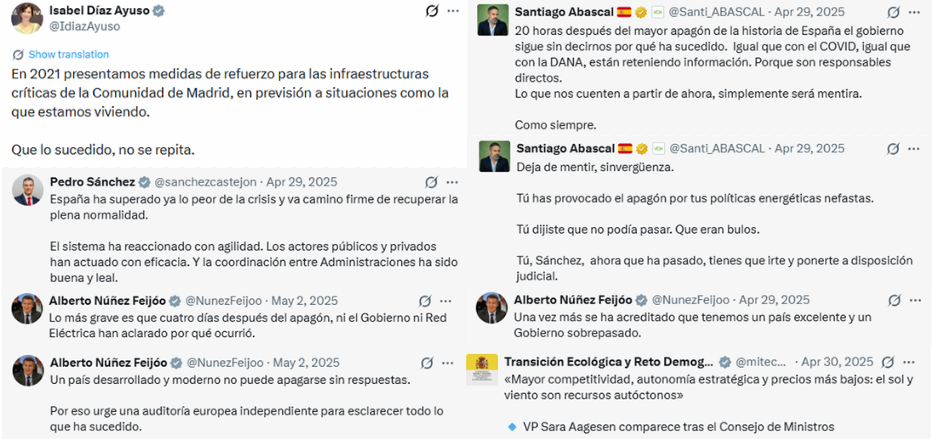
\includegraphics[width=\textwidth]{figuras/collage_politicos.png}
    \vspace{0.2cm}
    \caption[Reacciones de figuras políticas en X durante las
    72~horas posteriores al apagón.]{%
    Muestra representativa de publicaciones de líderes políticos
    españoles en la plataforma X durante las 72~horas posteriores
    al incidente.
    Fuente: capturas de X, elaboración propia}
    \label{fig:collage_politicos}
\end{figure}



% - - - - - - - - - - - - - - - - - - - - - - - - - - - - - - - - -
\subsection*{Síntesis: limitaciones estructurales ante incidentes
de alta complejidad técnica}
% - - - - - - - - - - - - - - - - - - - - - - - - - - - - - - - - -

El análisis permite identificar tres asimetrías estructurales en el
ecosistema digital ante un incidente de estas características: la
incompatibilidad temporal entre la velocidad de propagación viral y
la lentitud de la investigación forense técnica; la condición no
neutral del vacío informativo institucional, que es ocupado por
atribuciones causales prematuras; y la menor capacidad de difusión
algorítmica de la divulgación técnica frente a los mensajes de
indignación política \cite{gobierno2025,blackswan2025}.

Esta dinámica confirma que, ante disrupciones eléctricas de elevada
complejidad técnica, la comprensión pública del incidente queda
condicionada por los marcos interpretativos previos de cada agente
comunicativo, con independencia de la evidencia técnica disponible.
La consideración de este factor en el diseño de los protocolos de
comunicación de crisis de los operadores de sistemas críticos
constituye una de las lecciones operativas del 28 de abril de 2025.